\ifdefined\BuildingFromMainFile
\else
   \documentclass[../main.tex]{subfiles}
   \begin{document}
\fi


\graphicspath{{figure/}{../figure/}}

\onehalfspacing
\normalsize


\begin{abstract}   
\onehalfspacing
\small
Many genomic analyses start by aligning sequencing reads to a linear reference genome. However, linear reference genomes are imperfect, lacking millions of bases of unknown relevance, and are unable to reflect the genetic diversity of populations. This makes reference-guided methods susceptible to reference-allele bias. To overcome such limitations, we build a pangenome from six reference-quality assemblies from taurine and indicine cattle as well as yak. The pangenome contains an additional 70,329,827 bases compared to the \emph{Bos taurus} reference genome. Our multi-assembly approach reveals 30 and 10.1 million bases private to yak and indicine cattle, respectively, and between 3.3 and 4.4 million bases unique to each taurine assembly. Utilizing transcriptomes from 56 cattle, we show that the novel sequences encode transcripts that hitherto remained undetected from the \emph{Bos taurus} reference genome. We uncover novel genes, primarily encoding proteins contributing to immune response and pathogen-mediated immunomodulation, differentially expressed between \emph{Mycobacterium bovis}-infected and non-infected cattle that are also undetectable in the \emph{Bos taurus} reference genome. Using whole-genome sequencing data of cattle from five breeds, we show that reads which were previously misaligned against the bovine reference genome now align accurately to the novel sequences. This enables us to discover 83,250 polymorphic sites that segregate within and between breeds of cattle and capture genetic differentiation across breeds. Our work makes a so far unused source of variation amenable to genetic investigations and provides methods and a framework for establishing and exploiting a more diverse reference genome.

\medskip
\textbf{Keywords}: Genetic diversity, Genome graphs, Pangenome
\end{abstract}

\newpage

\section*{Significance}
% \doublespacing
\linespread{1.25}
Most sequence variant analyses rely on a linear reference genome that is assumed to lack millions of bases that occur in the genomes of other individuals. To quantify the extent and functional relevance of such missing bases, we integrate six genome assemblies from cattle and related species into a pangenome. This allows us to uncover more than 70 million bases that are not included in the \emph{Bos taurus} reference genome. Through complementary bioinformatics, genomics, and transcriptomics methods we discover novel genes that are differentially expressed and thousands of polymorphic sites that were unused so far. Our work provides a computational framework, broadly applicable to many species, to make a so far neglected source of genomic variation amenable to genetic investigations.

\section{Introduction}
 
\normalsize

A well-annotated reference genome enables systematic characterization of sequence variation within and between populations, as well as across species. The reference genome of domestic cattle (Bos taurus taurus) was generated from the inbred Hereford cow \emph{L1 Dominette 01449} \citep{rosen2020novo}. Long-read sequencing and sophisticated genome assembly methods have enabled spectacular improvements in the contiguity and quality of the \emph{Bos taurus} reference genome. The contig (contiguous sequence formed by overlapping reads without gaps) N50 size (i.e., 50\% of the genome is in contigs of this size or greater) of the bovine reference genome has increased from kilo- to megabases over the past five years \citep{rosen2020novo}. Recent method and sequencing technology developments have facilitated the assembly of multiple reference-quality genomes. The application of trio-binning \citep{koren2018novo} resulted in chromosome-scale haplotype-resolved assemblies for three taurine (Hereford, Angus, Highland cattle) and one indicine (Brahman) cattle breeds, as well as for yak (\emph{Bos grunniens}), a closely related species to domestic cattle \citep{low2020haplotype,rice2020continuous}.

DNA sequences from taurine and indicine cattle are typically aligned to the Hereford-based reference genome to discover and genotype variable sites. Reference-guided read alignment and variant genotyping has revealed millions of polymorphic variants that segregate within and between taurine and indicine cattle breeds \citep{kim2020mosaic,daetwyler2014whole,koufariotis2018sequencing}. However, using the linear reference in this alignment approach is susceptible to reference allele bias, particularly for DNA samples that are greatly diverged from the reference \citep{ballouz2019time,pritt2018forge}. Moreover, reference-guided methods are blind to variations in sequences that are not present in the reference genome \citep{wong2020towards}. Recent estimates suggest that millions of bases are missing in mammalian reference genomes \citep{sherman2019assembly,whitacre2015s}, indicating a high potential for bias.

Efforts to mitigate reference allele bias and increase the genetic diversity of reference genomes have led to graph-based references \citep{garrison2018variation,eggertsson2017graphtyper}. We have previously shown that a genome graph, which integrates linear reference coordinates and pre-selected variants, improves the mapping of reads and enables unbiased variant genotyping in different breeds of cattle \citep{crysnanto2019accurate,crysnanto2020bovine}. However, previous attempts focused on augmenting the \emph{Bos taurus} reference genome with small variations ($<$50bp), not the larger class of structural variations. Despite being an important source of genotypic and phenotypic diversity \citep{song2020eight,kehr2017diversity}, little is known about the prevalence and functional impact of structural variations in the cattle genome. The availability of reference-quality assemblies and long read sequencing data from different breeds of cattle now provides an opportunity to characterize sequence diversity beyond small variations \citep{hickey2020genotyping,li2020design}. 
In this paper, we integrate reference-quality assemblies from multiple taurine breeds as well as two close relatives into a multi-assembly graph with minigraph \citep{li2020design} (Table \ref{tab41:assemb}). We detect autosomal sequences that are missing in the \emph{Bos taurus} reference genome and investigate their functional significance using transcriptome data. We show that the non-reference sequences contain novel transcripts that are differentially expressed as well as polymorphic sites that segregate within and between breeds of cattle.

\bigskip

\begin{table}
    \centering
    \footnotesize
    \caption[Details of six bovine genome assemblies]{\textbf{Details of six bovine genome assemblies}} 
    \begin{tabular}{|l|l|l|l|l|l|l|l|} 
    \hline
    \multicolumn{1}{|c|}{Assembly (Species)}                                                  & \multicolumn{1}{c|}{Sex\textsuperscript{1}} & \multicolumn{1}{c|}{Primary data\textsuperscript{2}}            & \multicolumn{1}{c|}{\begin{tabular}[c]{@{}c@{}}Assembly \\type\end{tabular}} & \multicolumn{1}{c|}{Assembler} & \multicolumn{1}{c|}{\begin{tabular}[c]{@{}c@{}}Contig \\N50(Mb)\end{tabular}} & \multicolumn{1}{c|}{\begin{tabular}[c]{@{}c@{}}Scaffold \\N50(Mb)\end{tabular}} & \multicolumn{1}{c|}{\begin{tabular}[c]{@{}c@{}}Autosomes \\lengths (Gb)\end{tabular}}  \\ 
    \hline
    \begin{tabular}[c]{@{}l@{}}Hereford \\(\textit{Bos taurus taurus)}\end{tabular}           & F                                           & \begin{tabular}[c]{@{}l@{}}PacBio \\(80-fold CLR)\end{tabular}  & Primary                                                                      & Falcon                         & 21                                                                            & 108                                                                             & 2.489~                                                                                 \\ 
    \hline
    \begin{tabular}[c]{@{}l@{}}Angus\\(\textit{Bos taurus taurus)}\end{tabular}               & M                                           & \begin{tabular}[c]{@{}l@{}}PacBio \\(136-fold CLR)\end{tabular} & \begin{tabular}[c]{@{}l@{}}Haplotype\\resolved\end{tabular}                  & TrioCanu                       & 29.4                                                                          & 102.8                                                                           & 2,468~                                                                                 \\ 
    \hline
    \begin{tabular}[c]{@{}l@{}}Highland \\(\textit{Bos taurus taurus)}\end{tabular}           & F                                           & \begin{tabular}[c]{@{}l@{}}PacBio\\(125-fold CLR)\end{tabular}  & \begin{tabular}[c]{@{}l@{}}Haplotype\\resolved\end{tabular}                  & TrioCanu                       & 71.7                                                                          & 86.2                                                                            & 2,483                                                                                  \\ 
    \hline
    \begin{tabular}[c]{@{}l@{}}Original Braunvieh \\(\textit{Bos taurus taurus)}\end{tabular} & F                                           & \begin{tabular}[c]{@{}l@{}}PacBio \\(28-fold HiFi)\end{tabular} & Primary                                                                      & Hifiasm                        & 86.0                                                                          & 96.3                                                                            & 2,607                                                                                  \\ 
    \hline
    \begin{tabular}[c]{@{}l@{}}Brahman \\(\textit{Bos taurus indicus)}\end{tabular}           & F                                           & \begin{tabular}[c]{@{}l@{}}PacBio \\(136-fold CLR)\end{tabular} & \begin{tabular}[c]{@{}l@{}}Haplotype\\resolved\end{tabular}                  & TrioCanu                       & 23.4                                                                          & 104.5                                                                           & 2,478~                                                                                 \\ 
    \hline
    \begin{tabular}[c]{@{}l@{}}Yak \\(\textit{Bos grunniens)}\end{tabular}                    & F                                           & \begin{tabular}[c]{@{}l@{}}PacBio \\(125-fold CLR)\end{tabular} & \begin{tabular}[c]{@{}l@{}}Haplotype\\resolved\end{tabular}                  & TrioCanu                       & 70.9                                                                          & 94.7                                                                            & 2,478~                                                                                 \\
    \hline
    \end{tabular}
    \begin{flushleft}
    \textsuperscript{1} Female (F) and male (M) assemblies contain either X or Y chromosomal sequences. \\
    \textsuperscript{2} Additional data may have been used to polish the assemblies and facilitate scaffolding; CLR: continuous long reads; HiFi: high-fidelity.
    \end{flushleft}
    \label{tab41:assemb}
\end{table}

\section{Results}

\subsection*{Construction of a bovine multi-assembly graph}

We considered the Hereford-based Bos taurus reference genome and five reference-quality assemblies from three breeds of taurine (\emph{Bos taurus taurus}) cattle (Angus, Highland, Original Braunvieh) \citep{koren2018novo,low2020haplotype,rice2020continuous} and their close relatives Brahman (\emph{Bos taurus indicus}) \citep{low2020haplotype} and yak (\emph{Bos grunniens}) \citep{rice2020continuous}. All assemblies, except for the Original Braunvieh, were generated prior to this study. The reference-quality assembly for an Original Braunvieh female calf was created with 28-fold PacBio HiFi read coverage (see \emph{SI Appendix}, \ref{sup_not:s41}). The contig and scaffold N50 values of the six assemblies ranged from 21 to 80 Mb and 86.2 to 108 Mb, respectively Table \ref{tab41:assemb}.

\begin{figure}[!htb]
    \centering
    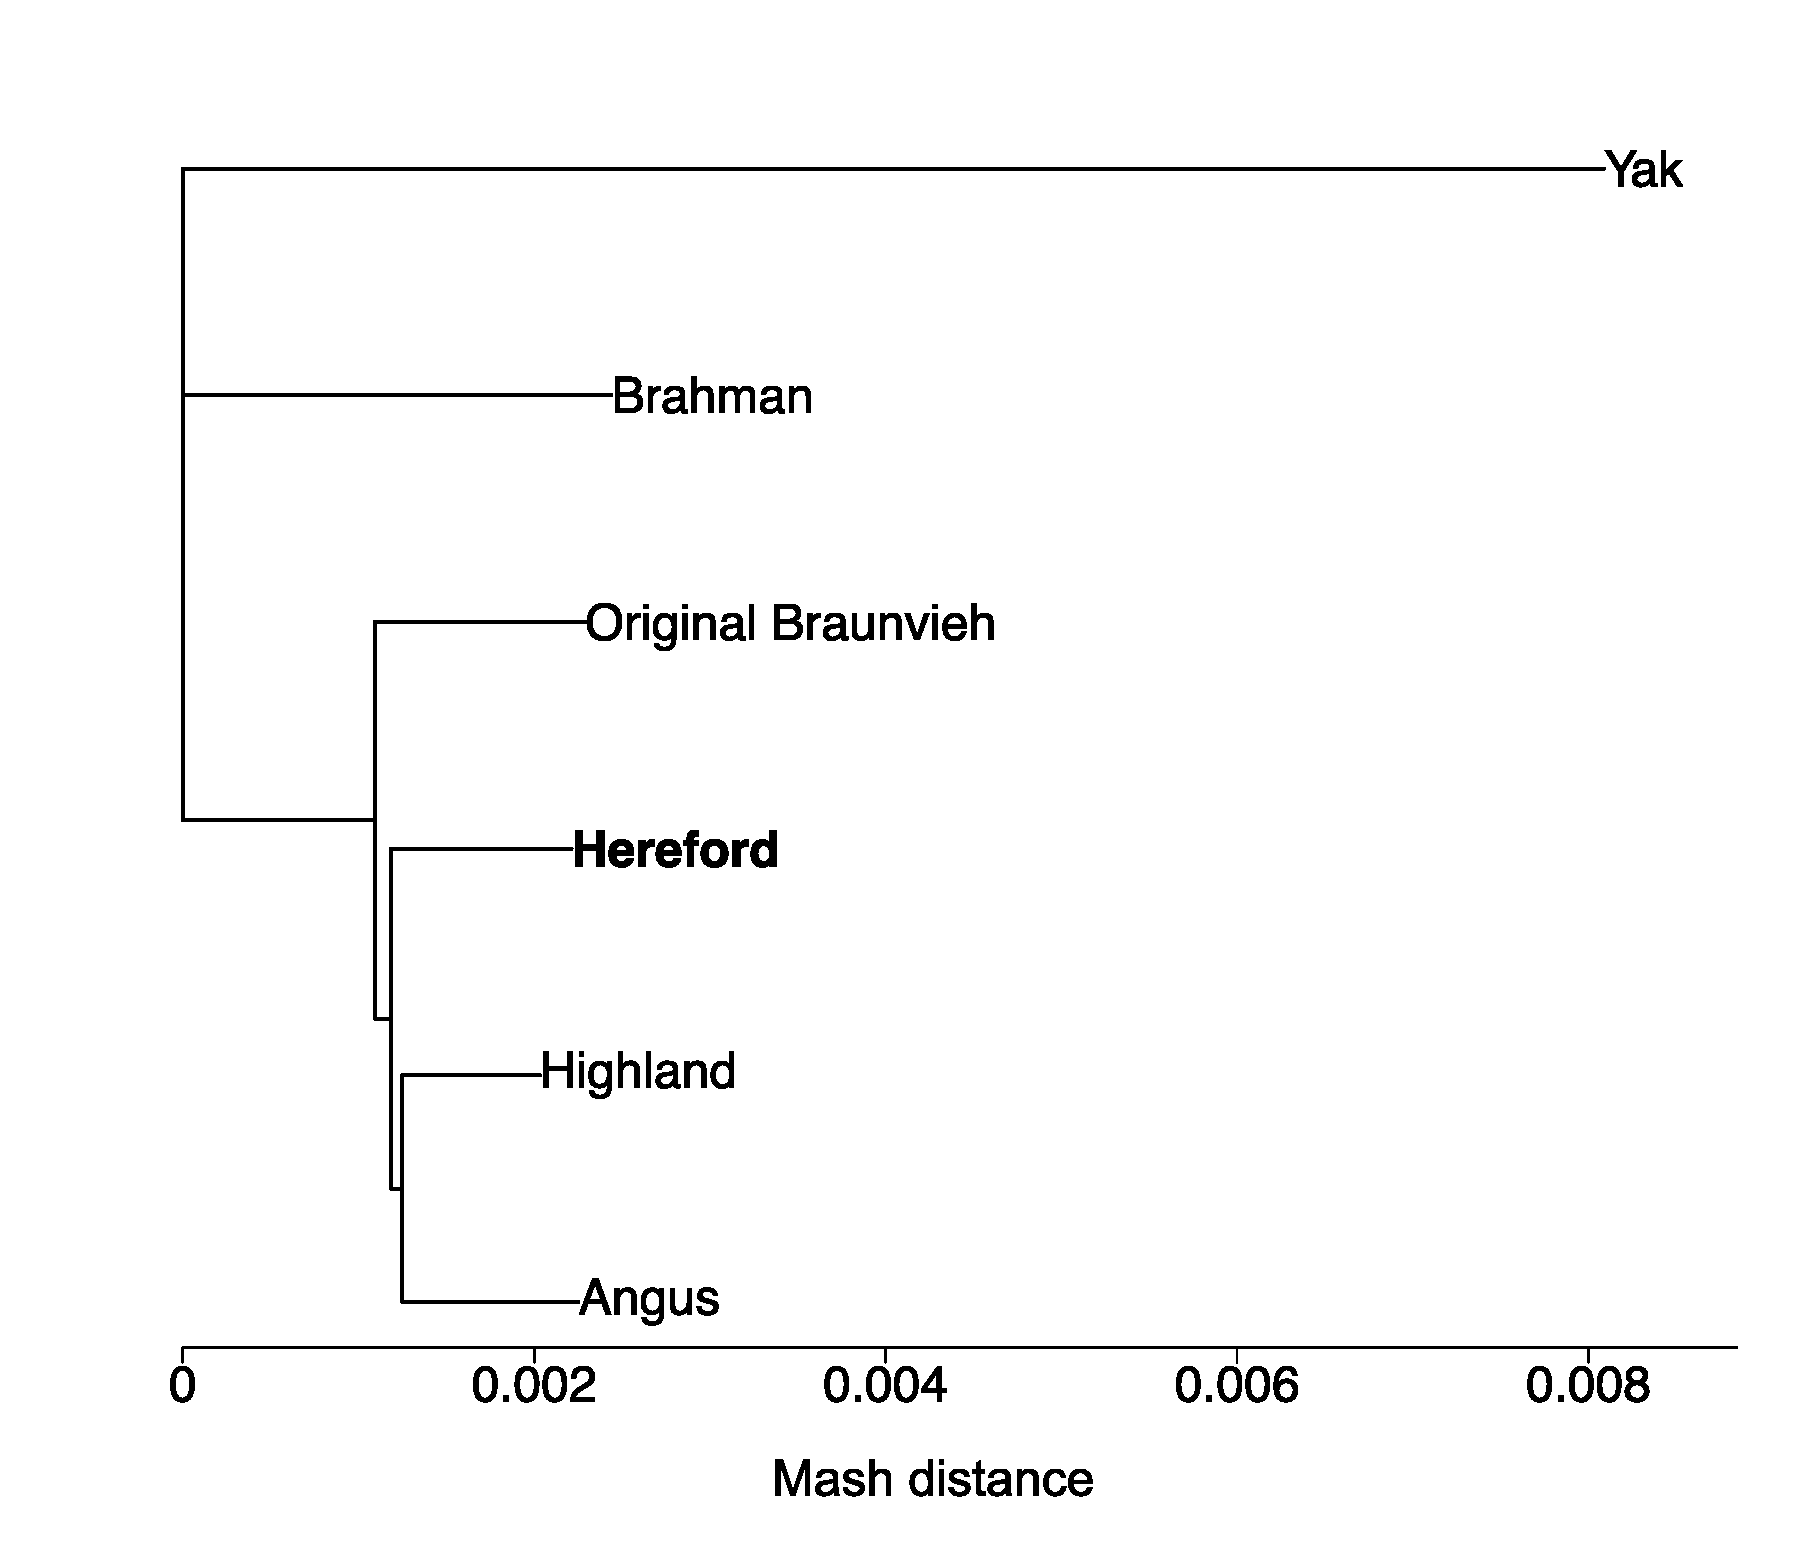
\includegraphics[width=\textwidth]{paper3/main_figure/Fig1.pdf}
        \caption[Phylogenetic bovine assemblies]{\textbf{Phylogenetic distance between six genome assemblies.} \\
        \footnotesize{A Mash-based phylogenetic tree derived from six bovine assemblies, including the current Hereford-based \emph{Bos taurus} reference genome (\textbf{bold}). The yak assembly was used as the outgroup to root the tree during building.}}
        \label{fig41:phylo}
\end{figure}


The six assemblies were integrated into a multi-assembly graph with minigraph. We only considered autosomal sequences because the haplotype-resolved assemblies represent either paternal or maternal haplotypes, thus lacking either X or Y chromosomal sequences. The Hereford-based linear reference genome (ARS-UCD1.2) formed the backbone of the bovine multi-assembly graph. The graph was then augmented with the five additional assemblies, added in order of increasing Mash-distance from the ARS-UCD1.2 reference \citep{ondov2016mash} Fig. \ref{fig41:phylo}. Constructing this multi-assembly graph took 4.1 CPU hours and 58 GB of RAM, taking 36 minutes of wall-clock time when using 10 threads.

\subsection*{Recovery of non-reference sequences from the multi-assembly graph}

Our bovine multi-assembly graph represents 2,558,596,439 nucleotides, spread across 182,940 nodes connected by 258,396 edges. On average, a node spans 13,985 nucleotides and is connected by 1.4 edges. Of the edges, 141,086, 113,332, and 3,978 connect two reference nodes, a reference and non-reference node, or two non-reference nodes, respectively. 

The vast majority (2,489,385,779 or 97.29\%) of nucleotides in the multi-assembly graph originate from the linear reference backbone, covered in 123,483 nodes. These reference nodes span 23,088 bases on average, ranging from 100 to 1,398,882 bases. The incremental integration of the Highland, Angus, Original Braunvieh, Brahman, and yak assemblies added 8,847, 4,613, 3,555, 11,996, and 30,446 non-reference nodes, respectively containing 14,679,286, 5,537,769, 7,013,258, 11,116,220, and 30,864,
127 non-reference bases. The resulting multi-assembly graph contained 59,457 non-reference nodes spanning 69,210,660 bases. 

To determine the support of the non-reference nodes, we aligned individual assemblies back to the multi-assembly graph. Nodes were then labelled according to which assembly path traversed them (see \emph{SI Appendix}, Figs. \ref{sup_fig:s41} \& \ref{sup_fig:s42}). This approach enabled a straightforward confirmation of minigraph’s mapping accuracy. Only reference nodes should contain a Hereford label, since this assembly was used as the backbone of the graph. Mapping was highly accurate, as indicated by an F1 score of 99.97\%.

The non-reference nodes of the multi-assembly graph had a cumulative length of 43,341,418, 23,644,772, 18,202,102, 14,453,112 and 15,542,368 bases in the yak, Brahman, Original Braunvieh, Angus, and Highland assemblies. Yak and Brahman non-reference nodes were shorter on average compared to the taurine assemblies (\emph{SI Appendix}, Fig. \ref{sup_fig:s43}). Most non-reference nodes (41,855 or 70.40\%) and non-reference sequences (42.52 Mb, 69.52\%) were either private to yak (29,854 nodes, 29.9 Mb), Brahman (7,843 nodes, 8.22 Mb), or shared by both assemblies (4,158 nodes, 3.05 Mb). The Original Braunvieh, Highland, and Angus assemblies contributed 4.51, 2.78 and 2.39 Mb in 2,016, 1,938 and 1,759 nodes, respectively, that were not detected in any other assembly. The three taurine assemblies shared 668 nodes containing 0.77 Mb not detected in ARS-UCD1.2, yak, or Brahman. There were also 1,318 non-reference nodes with a cumulative length of 4.4 Mb supported by all five additional assemblies.

The core genome of the multi-assembly graph (i.e., nodes shared by all assemblies) is contained in 67,482 nodes with a cumulative length of 2,402,561,410 bases. About 6.10\% of the pangenome (115,458 nodes containing 156,035,029 bases) is flexible (i.e., not shared by all assemblies). Of the flexible part, 69,697 nodes containing 97,106,100 bases are shared by at least two assemblies, and 45,761 nodes with 58,928,929 bases are only found in one assembly. The profile of the multi-assembly graph changes markedly when distant assemblies (e.g., Brahman, yak) are added (\emph{SI Appendix}, \ref{sup_not:s42}).

The minigraph approach used to construct the multi-assembly graph does depend on an initial sequence forming a backbone. The choice of backbone consequently impacts the amount of non-reference sequence detected from each additional assembly (see \emph{SI Appendix}, \ref{sup_not:s43}). However, the overall effect on the sequence content of the multi-assembly graph is relatively minor, with 68.72±3.17 Mb of non-reference sequence identified across all possible backbones.

\subsection*{Structural variation discovery from the multi-assembly graph}

Using the bubble popping algorithm of gfatools \citep{li2020design}, we identified 68,328 structural variations present in the multi-assembly graph. To reveal true alleles within these structural variations, we traversed all possible paths through the bubbles (i.e., alleles) and retained only those that were supported by at least one assembly (\emph{SI Appendix}, Fig. \ref{sup_fig:s42}). Most of the structural variations had two alleles (64,224 or 94\%). The remaining 4,104 structural variations were multi-allelic, most of which had three alleles (3,324 or 81\%). We identified 141,747 alleles at the structural variations, including 73,506 non-reference alleles with a cumulative length of 74,453,929 bases.  

We overlapped the breakpoints of the structural variations with the Ensembl annotation (build 101) of ARS-UCD1.2. Almost all structural variations are either intergenic (47,642 or 69.81\%) or intronic (20,227 or 29.64\%). There were 170 and 202 exons and coding sequences, respectively, of 338 unique genes affected by structural variations. A Panther GO-Slim Biological Process \citep{mi2019panther} analysis indicated that these genes are enriched for genes related to the adaptive immune response (4.35$-$fold, P$=$0.04), T-cell mediated immunity (6.37$-$fold, P$=$0.04), actin filament depolymerization (8.54$-$fold, P$=$6.56e$-$03), microtubule cytoskeleton organization (10.48$-$fold, P$=$1.85e$-$04), and iron-sulfur cluster assembly (9.96$-$fold, P$=$0.02). 

The non-reference alleles consisted of 40,369 insertions and 33,137 deletions with an average length of 1,181 and 1,210 bases respectively (\emph{SI Appendix}, Table \ref{sup_tab:s41}). The cumulative length (absolute difference between reference and non-reference allele) was longer for insertions (47,691,942 bases) than deletions (40,101,303 bases). This pattern was similar for biallelic variations (35,748 and 28,476 biallelic insertions and deletions, respectively, encompassing 37,388,222 and 28,373,582 bases with an average variant length of 1,045 and 996 bases). The multi-assembly graph contained more complete insertions (20,432; i.e., only non-reference sequences present in the bubbles, thus reference length is 0) than alternate insertions (15,316; i.e., both reference and non-reference sequences present but non-reference allele is longer). The pattern was similar for deletions. The multi-allelic structural variations had 13,299 alleles including 9,282 non-reference alleles with 4,621 insertions and 4,661 deletions, respectively, affecting 11,727,721 and 10,303,720 bases. Bubbles with multi-allelic structural variations contained more mixed mutations (1,941; both deletions and insertions detected within the same bubble) than multiple mutations of the same type (994 and 1,082 for multiple insertions and deletions, respectively). 

When compared to the ARS-UCD1.2 backbone, the yak, Brahman, Original Braunvieh, Angus, and Highland assemblies contained respectively 49,836, 22,976, 10,965, 10,735, and 10,560 non-reference alleles (Fig. \ref{fig42:nrfsec}). Most non-reference alleles (36,443, total length: 30 Mb) were private to the yak assembly. We detected 9,267, 2,232, 2,133, and 2,037 non-reference alleles, respectively, containing 10.1, 4.9, 3.8, and 3.3 Mb that were private to the Brahman, Original Braunvieh, Highland, and Angus assembly (Fig. \ref{fig42:nrfsec}, \emph{SI Appendix}, Fig. \ref{sup_fig:s45}). We also found 1,749 alleles within the 4.4 Mb of non-reference sequence (2.1 Mb of which is non-repetitive) shared by all assemblies except ARS-UCD1.2.

We mapped PacBio HiFi reads from a Nellore (\emph{Bos taurus indicus}) x Brown Swiss (\emph{Bos taurus taurus}) crossbred bull to the multi-assembly graph to examine support for the non-reference alleles. Nearly one third of the structural variation breakpoints had support from the hybrid cattle, while this rose to approximately three-quarters after excluding nodes with only yak labels. Since neither parental breed is present in the multi-assembly graph, this suggests that the discovered structural variation may be prevalent in different breeds of taurine and indicine cattle. 

\begin{landscape}
    \begin{figure}[!htb]
        \centering
        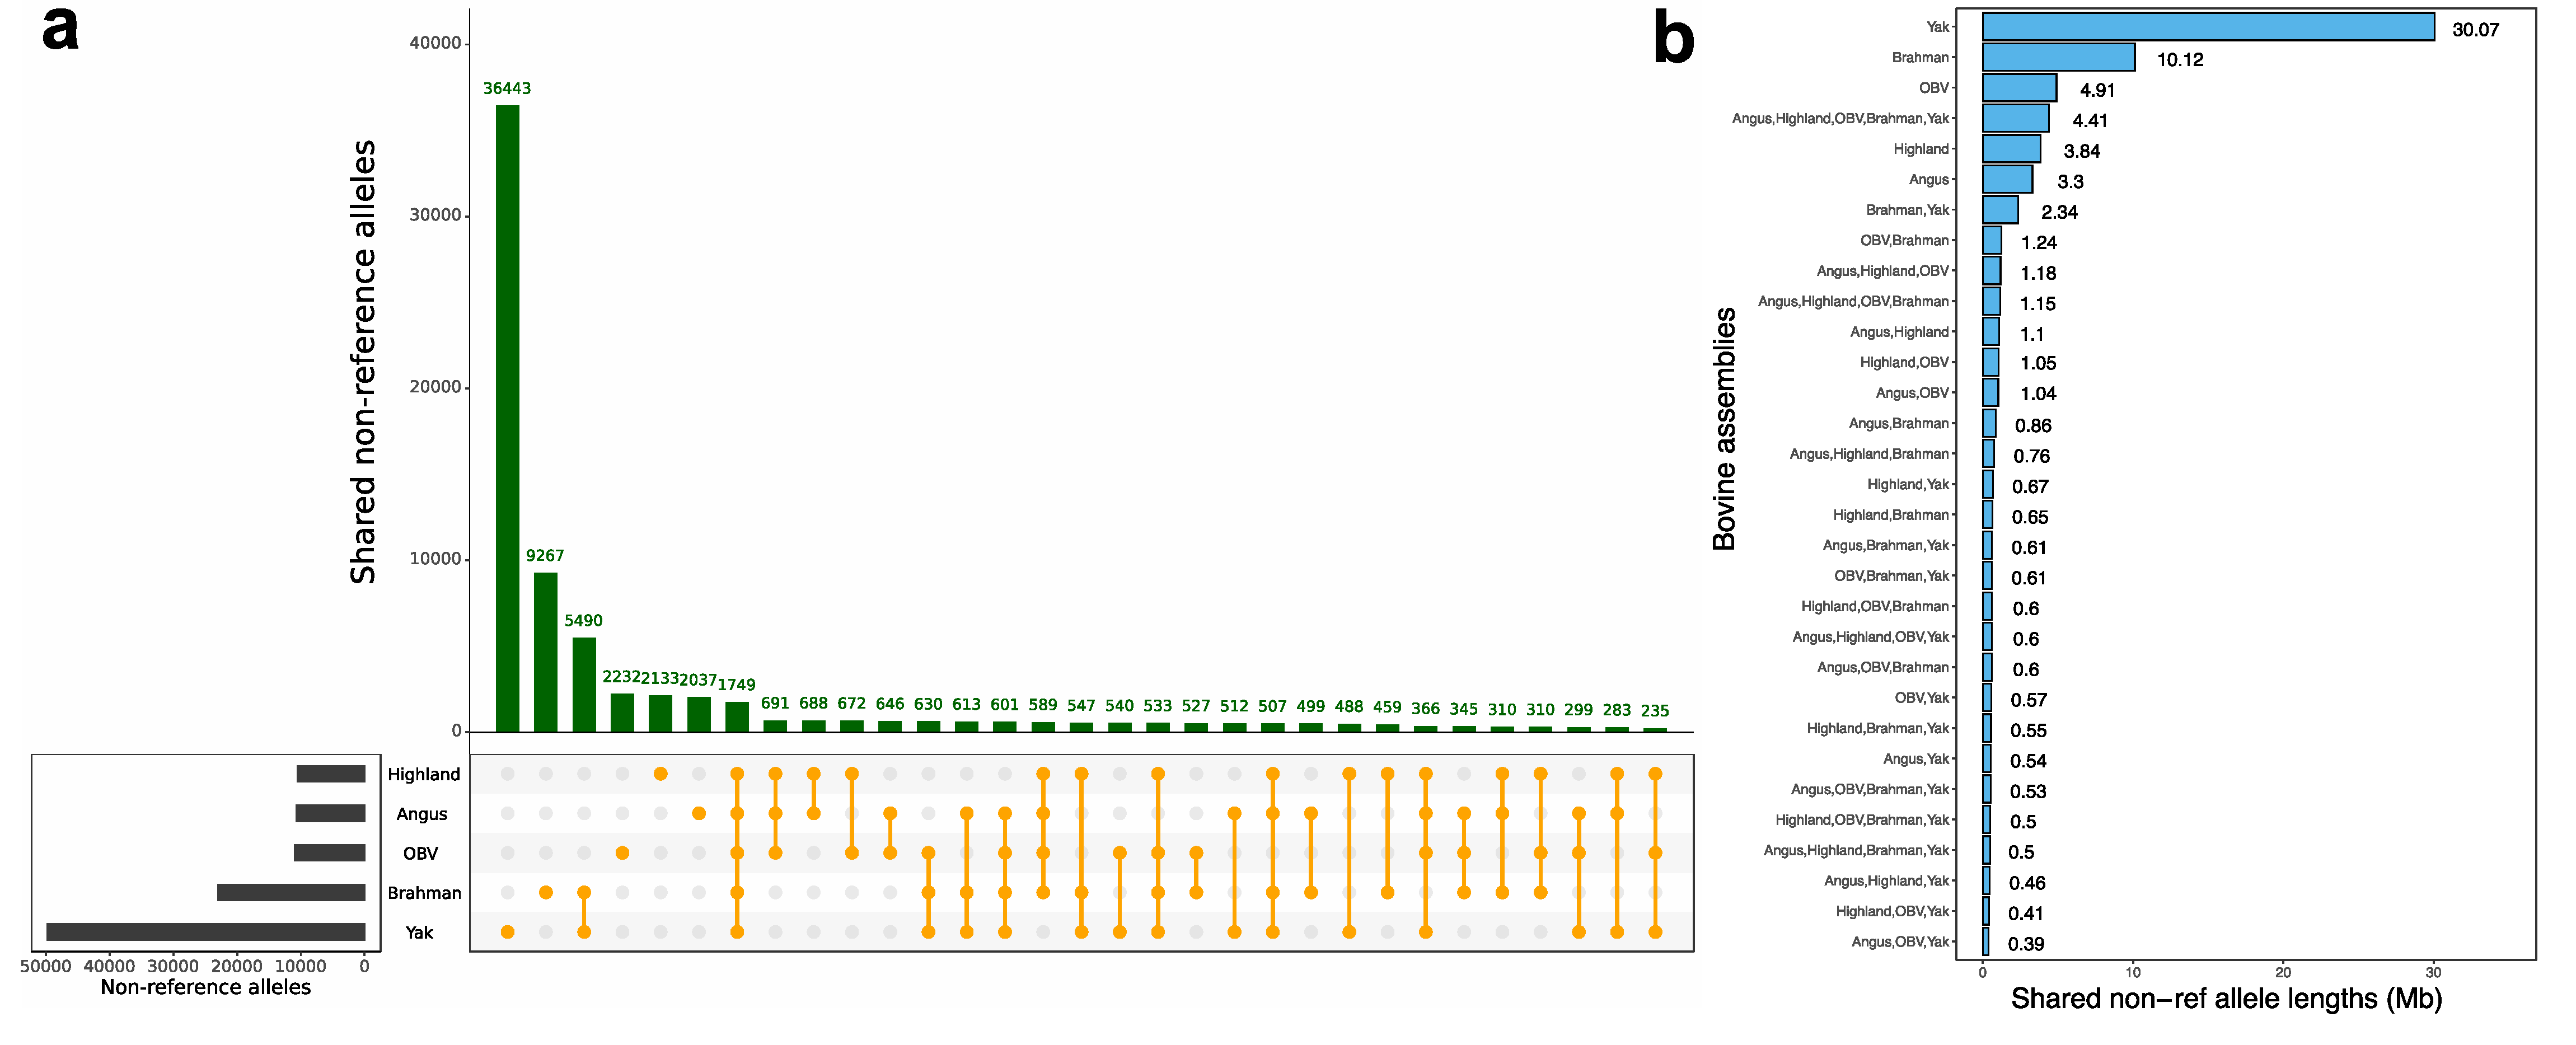
\includegraphics[width=1.5\textwidth]{paper3/main_figure/Fig2.pdf}
            \caption[Sharing non-reference alleles]{\textbf{Non-reference alleles detected across assemblies.} \\
            \footnotesize{Intersection of non-reference alleles \textbf{(a)} and cumulative length of the alleles \textbf{(b)} found in five assemblies when compared to ARS-UCD1.2. OBV = Original Braunvieh.}}
            \label{fig42:nrfsec}
    \end{figure}  
\end{landscape}


\subsection*{Sequence content of the structural variations}

In order to investigate the functional relevance of the non-reference sequences, we extracted 45,357 non-reference alleles from the 70,329,827 non-reference bases in the multi-assembly graph (\emph{SI Appendix}, Fig. \ref{sup_fig:s46}). These sequences originate from 38,906 biallelic and 6,451 multiallelic structural variations, respectively, that have a cumulative length of 43,003,591 and 27,326,236 bases. On average, the alleles of multiallelic structural variations were four times longer than that of biallelic bubbles (4,205 versus 1,104 bases). 
 
The non-reference sequences are largely comprised of repetitive elements (53,690,260 bases or 76.34\%, \emph{SI Appendix}, Fig. \ref{sup_fig:s47}). LINE/L1 and LINE/RTE-BovB account for 28.04 (52.22\%) and 6.77 (12.61\%) Mb repetitive non-reference bases, respectively. Repetitive sequences (both interspersed and simple repeats) are more evenly distributed across the autosomes than non-repetitive sequences. Both repetitive and non-repetitive non-reference sequences were detected at two regions on bovine chromosomes 18 and 23 that encompass the leukocyte receptor complex and the major histocompatibility complex (\emph{SI Appendix}, Fig. \ref{sup_fig:s48}). 

We hypothesized that the 16,639,567 non-repetitive non-reference bases contain transcribed sequences. A BLASTX search of these sequences against a protein sequence database of Bos and related species revealed hits for 403 structural variations containing 299,337 non-reference bases. As a complementary approach, we predicted genes from the non-repetitive sequences using the Augustus software tool. The \emph{ab initio} prediction revealed 857 gene models from 768 distinct structural variations that had a minimum coding sequence length of 150 bp, including 374 complete gene models with transcription start site, start codon, exons, stop codon, and transcription termination site (\emph{SI Appendix}, Table \ref{sup_tab:s42}). On average, the transcript, coding sequence, and protein length of the complete gene models is respectively 4,742 bp, 794 bp, and 264 aa. 

\subsection*{\emph{De novo} transcript assembly from the non-reference sequences}

As the two complementary gene prediction methods indicated that the novel sequences contain transcribed features, we sought experimental evidence. We appended the 70 Mb of repeat masked non-reference sequences contained in 45,357 additional contigs to the ARS-UCD1.2 reference, making an extended reference genome. This renders the non-reference sequences amenable to current methods of linear mapping of transcriptome data. Using HISAT2, we aligned liver transcriptomes from 39 cattle across taurine (Angus, Holstein, Jersey) and indicine (Brahman) breeds to both the linear reference as well as the extended reference. We also aligned transcriptomes from Dominette, the animal sequenced to assemble the \emph{Bos taurus} reference genome. A greater portion of reads mapped to the extended reference compared to the original reference for all examined samples (\emph{SI Appendix}, Fig. \ref{sup_fig:s49}). Across the 40 samples, the overall mapping rate increased by 0.037\%, which corresponds to approximately 18K reads for a paired-end RNA-seq dataset of 25 million reads. The mapping improvements were larger for samples with great genetic distance from the reference genome. Brahman had the largest improvement (0.060\%), followed by the taurine breeds: Angus (0.032\%), Holstein (0.026\%), and Jersey (0.030\%). As expected, Dominette benefitted the least (0.010\%), but still demonstrated an improvement over using the original reference. 

Next, we used StringTie2 \citep{kovaka2019transcriptome}, guided with gene models predicted by Augustus (see above), to assemble reads which aligned to non-reference sequences into 1,431 putatively novel genes. Of these, 885 were expressed at TPM ≥ 1 in at least one breed, including 405 that were originally predicted by Augustus. We selected these 405 putatively novel genes, supported by both \emph{ab initio }prediction and \emph{de novo} transcript assembly for further analyses. 

Only 263 of the 405 putatively novel genes were expressed at TPM ≥ 1 in Dominette, with BLASTP queries indicating they may be divergent copies of ribosomal proteins or olfactory receptors. The remaining 142 putatively novel genes were expressed at TPM ≥ 1 in Angus, Holstein, Jersey or Brahman cattle. Most were expressed in Brahman cattle (Fig. \ref{fig43:rnanov}a), including 20 putatively novel genes specific to this indicine breed. Among the taurine breeds, Angus contributed more putatively novel genes than either Holstein or Jersey cattle. Putatively novel genes common to all four non-reference breeds accounted for nearly half, 68 of the 142, identified in any non-reference breed (Fig. \ref{fig43:rnanov}b). The average expression was significantly higher (P=0.004, one-tailed t-test) for genes that were expressed in at least two breeds (N=106, TPM=13.48) than genes expressed in only one breed (N=36, TPM=1.64). BLASTP queries provided additional support for 57 out of 142 putatively novel genes (\emph{SI Appendix}, Fig. \ref{sup_fig:s410}). The top hits suggest that the putatively novel genes encode proteins related to: immune response (antigen-presenting glycoprotein, immunoglobulin, BOLA, killer-T-cell, interferon, Ig-like lectin, CMRF35, MHC, cytokine), signalling (G-protein signalling protein, tyrosine-phosphatase), cytoskeleton regulations (myosin, actin, twinfilin, KANTB1), lipid metabolism (apolipoprotein, lipid-binding protein), and protein modifications (heat-shock chaperone, ubiquitin conjugating enzyme, rhoA ubiquitin). 



\begin{figure}[!htb]
    \centering
    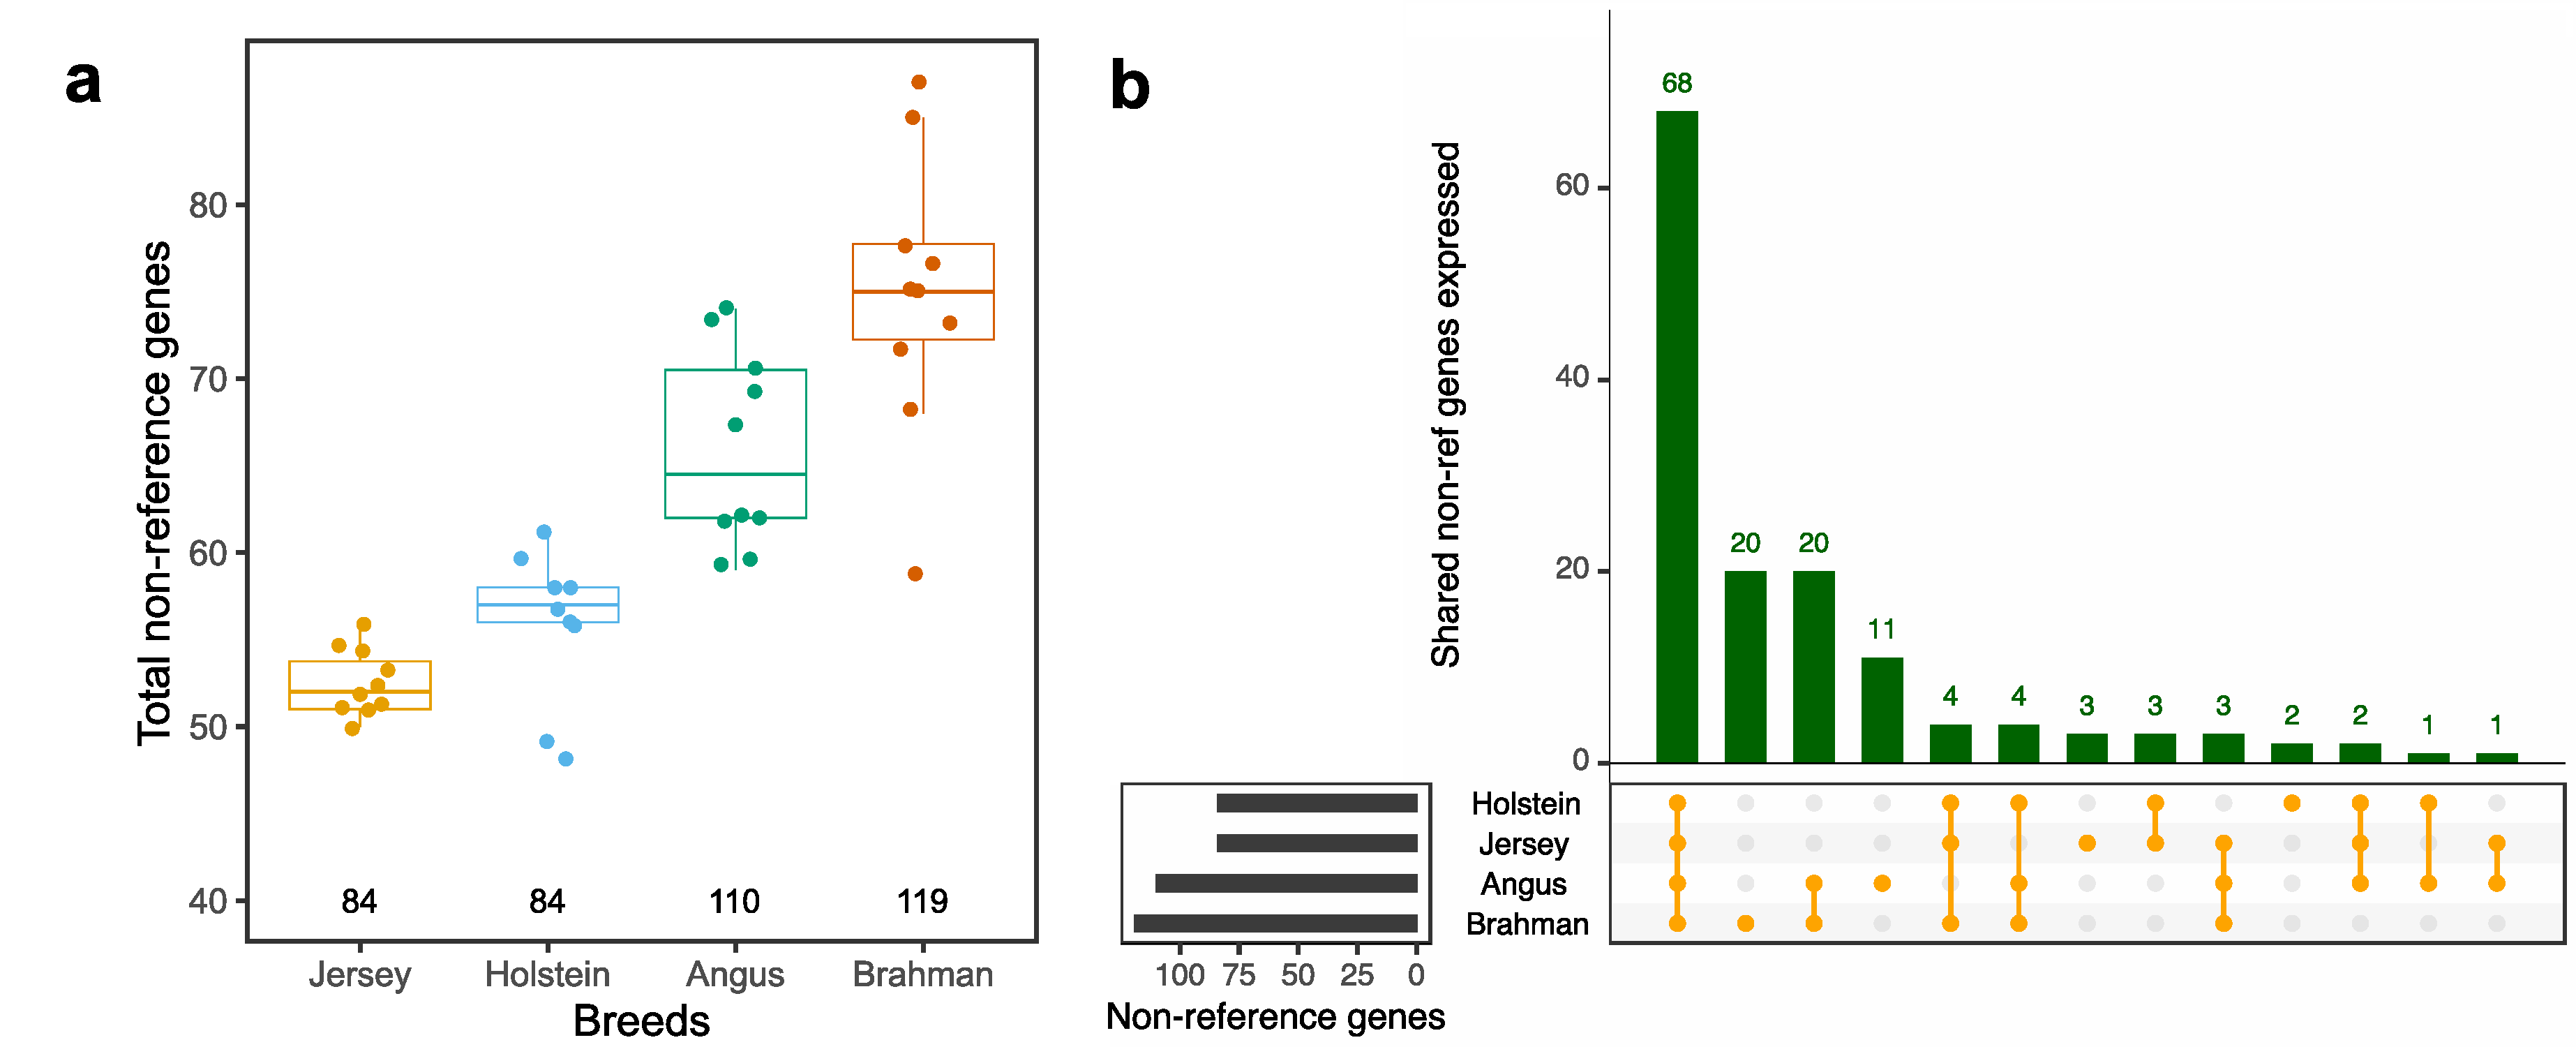
\includegraphics[width=\textwidth]{paper3/main_figure/Fig3.pdf}
        \caption[Transcription of novel genes]{\textbf{Novel transcribed genes detected from non-reference sequences.} \\
        \footnotesize{\textbf{(a)} Number of non-reference genes expressed ≥1 TPM in liver tissue from taurine (Jersey, Holstein, Angus) and indicine (Brahman) cattle breeds. Each point represents the number of novel genes detected per animal. The number of distinct novel genes detected for each breed is indicated below the boxplots. \textbf{(b)} Expression of 142 putatively novel non-reference genes in the four cattle breeds.}}
        \label{fig43:rnanov}
\end{figure}

\subsection*{Non-reference sequences contain differentially expressed genes}

To investigate if the non-repetitive sequences also encode transcripts that are differentially expressed between individual \emph{Bos taurus} cattle, we obtained publicly available peripheral blood leukocyte transcriptome data for eight \emph{Mycobacterium} bovis-infected and eight non-infected Holstein cattle \citep{mcloughlin2014rna}. Following the transcriptome analysis introduced earlier, the RNA sequencing reads were aligned to both the standard and extended ARS-UCD1.2 reference genome sequence. Between 8,616,414 and 23,940,699 RNA sequencing reads aligned to the standard and between 8,631,277 and 23,977,859 RNA sequencing reads aligned to the extended reference genome. The subsequent \emph{de novo} transcript assembly from the non-reference sequences produced 949 transcripts, encoded by 661 putatively novel genes. We appended them to the Ensembl ARS-UCD1.2 annotation, yielding a total of 28,268 genes. Considering only unique alignments, we detected expression levels $≥$ 1 CPM in at least eight samples for 13,085 genes, including 272 novel genes. We subsequently tested these genes for differential expression, finding 3,646 genes, including 36 putatively novel genes, which were differentially expressed (FDR ≤ 0.05) between \emph{Mycobacterium bovis}-infected and non-infected cattle (Fig. \ref{fig44:rnadif}a). The top differentially expressed genes from our extended Ensembl ARS-UCD1.2 annotation, as well as their transcript abundances in cases and controls, agreed well with the original findings from \citet{mcloughlin2014rna} that were based on the previous UMD3.1 annotation (Pearson R log2FC: 0.99) as well as with those from the standard ARS-UCD1.2 reference genome annotation (Pearson R log2FC: 0.99, \emph{SI Appendix}, \ref{sup_not:s44}). 


Within the 36 putatively novel differentially expressed genes, 28 and 8 are respectively up- and downregulated in peripheral blood leukocytes of \emph{Mycobacterium bovis}-infected cattle, with an average 2-fold change compared to non-infected controls (\emph{SI Appendix}, Fig. \ref{sup_fig:s411}). Multidimensional scaling representations of transcript abundance estimates of the 36 differentially expressed genes separated \emph{Mycobacterium bovis}-infected from non-infected cattle (Fig. \ref{fig44:rnadif}b). BLASTX queries against a protein reference database provided additional support for 13 out of 36 differentially expressed genes (\emph{SI Appendix}, Table \ref{sup_tab:s43}). The top upregulated non-reference gene supported by the BLASTX query (4.04-fold increase, \emph{P}$=$1.98e-05) encodes the Workshop Cluster (WC) 1.1-like protein, i.e., a receptor expressed on gamma delta T cells that modulates the immune response to \emph{Mycobacterium bovis} infections \citep{mcgill2014specific,damani2018variegated,kennedy2002modulation}. 

The top downregulated non-reference gene supported by the BLASTX query encodes a protein with high similarity (79.80\%) to leukocyte immunoglobulin-like receptor A5 (LILRA5). LILRA5 triggers the strength of the innate immune response to \emph{Mycobacterium} infections \citep{bah2018meta} and might serve as a target for pathogen-mediated immunomodulation. Many genes of the leukocyte receptor complex are missing in the assembled chromosomes of the ARS-UCD1.2 reference \citep{bakshy2021development}; instead, \emph{LILRA5} (LOC100139766) is annotated on a 236 kb long unplaced scaffold (NW\_020190675). A non-reference gene encoding a protein similar to \emph{LILRA5} is located within a 20.4 kb insertion of the multi-assembly graph at 62,471,732 bp on chromosome 18. Both taurine (Original Braunvieh) and indicine (Brahman) assemblies support this insertion. The putatively novel gene encoding \emph{LILRA5} is expressed at 9.59$±$2.54 and 23.10$±$8.30 CPM, respectively, in \emph{Mycobacterium bovis}-infected and non-infected cattle, corresponding to a 2.19$-$fold decrease (\emph{P}$=$1e-04) in infected cattle (\emph{SI Appendix}, Table \ref{sup_tab:s43}).

\begin{figure}[!htb]
    \centering
    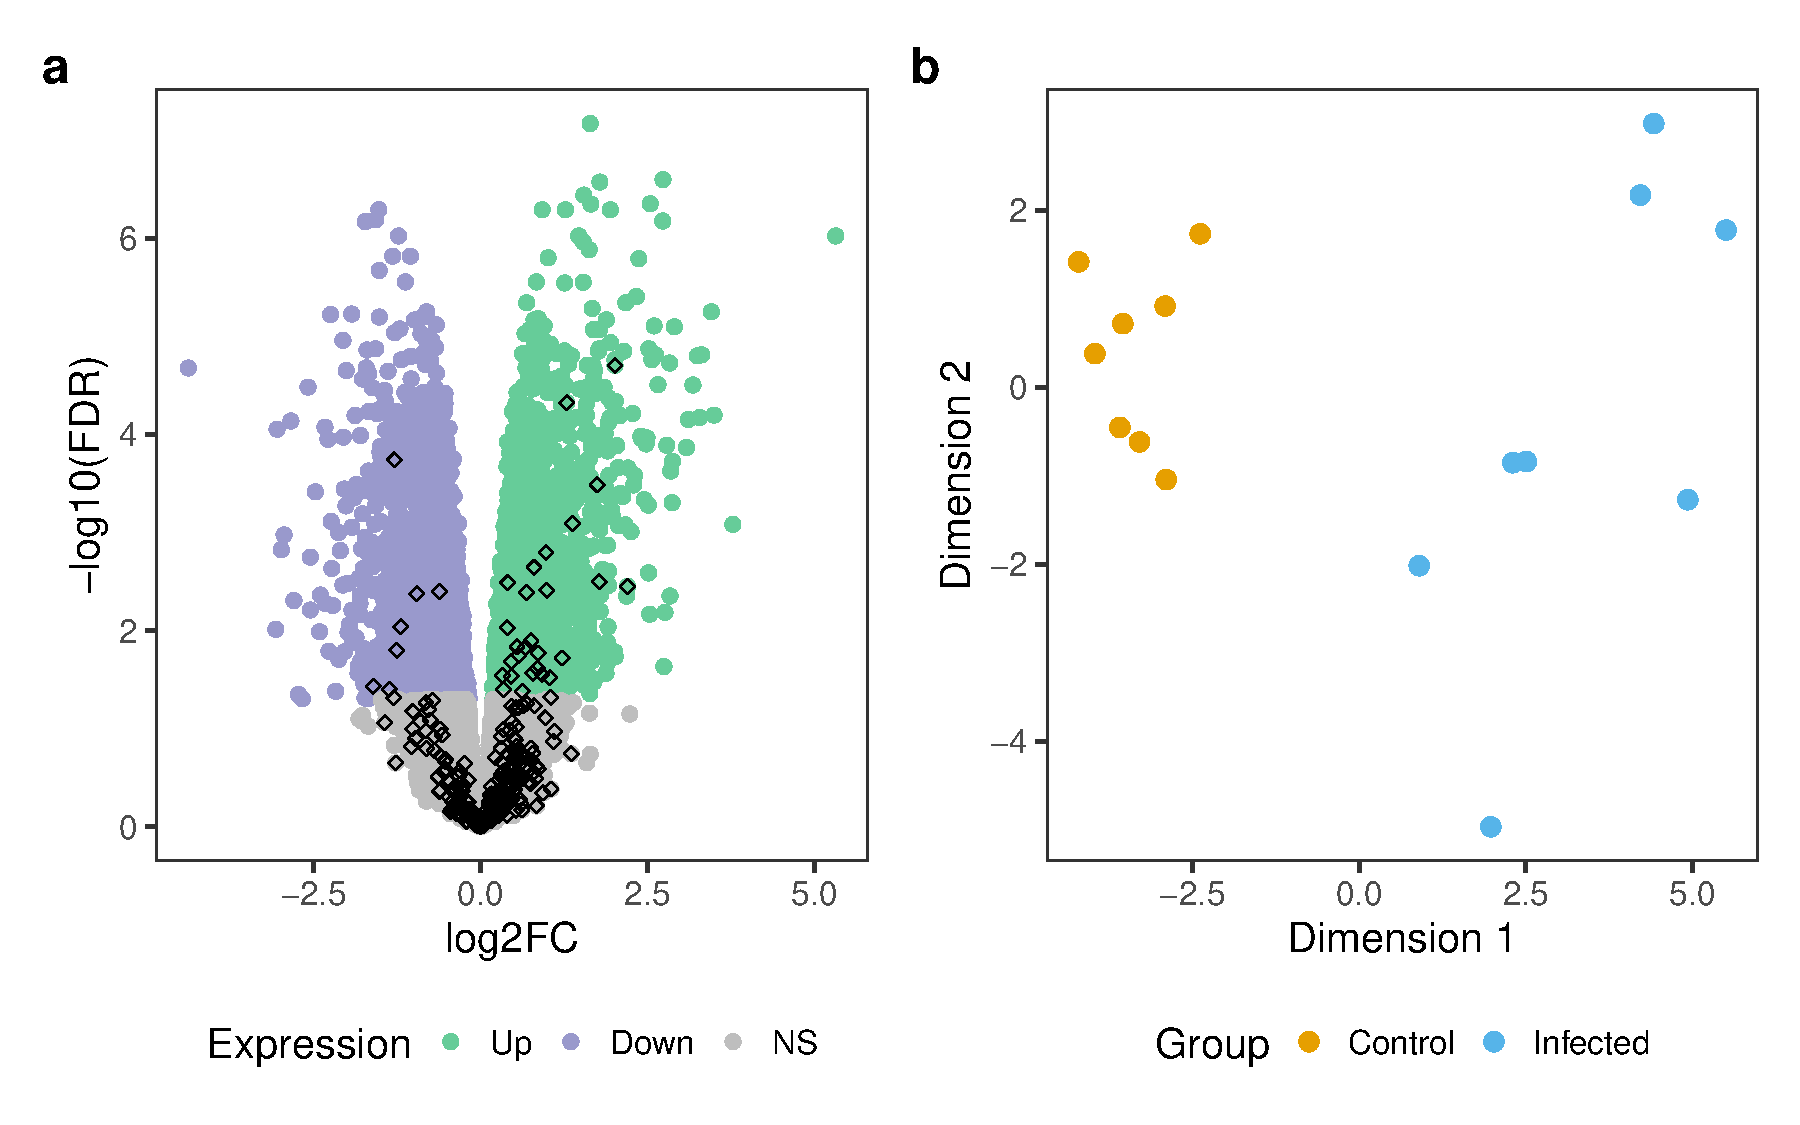
\includegraphics[width=\textwidth]{paper3/main_figure/Fig4.pdf}
        \caption[Differential expression of novel genes]{\textbf{Differentially expressed non-reference genes.} \\
        \footnotesize{\textbf{(a)} Volcano plot representing results from the differential expression analysis. Green and purple color indicates genes that are up- and downregulated (FDR ≤ 0.05), respectively, in peripheral blood leukocytes of \emph{Mycobacterium bovis}-infected cattle. Diamond shapes indicate the 272 putatively novel genes found in non-reference sequences. \textbf{(b)} Multidimensional scaling plot of 36 differentially expressed non-reference genes in \emph{Mycobacterium bovis}-infected (blue) and non-infected (orange) Holstein cattle.}}
        \label{fig44:rnadif}
\end{figure}


\subsection*{Variant discovery from the non-reference sequences}

Next, we mapped short sequencing reads, with an average of 19-fold sequencing coverage, from 45 cattle representing five taurine breeds against ARS-UCD1.2 and the extended ARS-UCD1.2 reference genome. An average number of 34,342 reads per sample mapped perfectly within 50 bp of the breakpoints of the newly added contigs indicating that the addition of 100 bp flanking sequence was sufficient to facilitate accurate alignments. Across 45 samples, the average mapping rate increased by 0.0176\% over ARS-UCD1.2, corresponding to approximately 100K sequencing reads for a DNA sample sequenced at 30-fold coverage. The mapping rate increased more noticeably for Brown Swiss (0.024\%) and Original Braunvieh (0.021\%) than Holstein (0.015\%) and Simmental (0.016\%) cattle (\emph{SI Appendix}, Fig. \ref{sup_fig:s412}). Similarly, to the transcriptome mapping, sequence reads from Dominette benefitted the least from the extended reference genome (0.006\%). However, the increase in mapping rate was greater (0.013\%) for other Hereford cattle. For all breeds, the extended reference genome also enabled more perfect alignments (alignments without difference from the reference), less partially mapped (i.e., clipped) reads, and less reads with supplementary alignments. However, the proportion of reads with unique alignment was lower for the extended than standard reference genome (\emph{SI Appendix}, Table \ref{sup_tab:s44}). 

We next investigated the alignments against the 2,115,702 non-repetitive non-reference bases detected in all assemblies except ARS-UCD1.2. Among these, 919,761 bases were covered by confident alignments (≥10-fold) from Dominette. This suggests that, although absent from the autosomal assembly, these sequences do occur in the animal used to construct the reference. However, 1,195,941 bp were not covered with reads from Dominette, but instead from Brown Swiss, Holstein, Original Braunvieh or Simmental samples. Strikingly, reads from non-Dominette Hereford samples covered 745,392 of the 1,195,941 bases. This directly implies that Dominette has individual-specific deletions, which are either rare or absent in other Hereford cattle.

Mapping against the extended reference resulted in many reads changing alignment location to the non-reference additions. Most (85.55\%) of the reads mapping at non-reference sequences already mapped to the original ARS-UCD1.2 reference genome, although 5\% of these mapped to unplaced contigs, while 14.45\% were previously unmapped. These mappings displayed an increase in the average mapping quality (22 to 44), alignment score (110 to 142), and alignment identity (0.975 to 0.995). The proportion of clipped reads decreased from 39\% to 4\%. The subset of these reads which were previously unmapped showed even greater improvements (\emph{SI Appendix}, Fig. \ref{sup_fig:s413}).

Using reads with mapping quality greater than 10 for reference-guided sequence variant genotyping yielded 83,250 filtered variants (73,709 SNPs, 9,541 Indels) in non-reference sequences that were identified by both \emph{SAMtools} and \emph{GATK}. These variants formed 80,995 biallelic and 2,255 multi-allelic sites, with a Ti:Tv ratio of 1.91, averaging 1.18 variants per kb. 3890 small variations (Ti:Tv ratio: 1.79) were detected within 50 bp of the breakpoints of the newly added contigs. On average each Brown Swiss, Original Braunvieh, Holstein, Simmental, and Hereford animal respectively had 31,028, 29,685, 29,851, 30,309, and 15,845 variant sites in non-reference bases (Fig. \ref{fig45:varnrf}a). A DNA sample from Dominette had considerably fewer polymorphic sites at non-reference bases, only 7,531. Most variants (32.67\%) had alternate allele frequency less than 0.1, and 193 were fixed for the alternate allele (\emph{SI Appendix}, Fig. \ref{sup_fig:s414}). The top principal components from a genomic relationship matrix that was built from the 83,250 non-reference variants separated the animals by breeds (Fig. \ref{fig45:varnrf}b,c). Functional annotation based on the gene models predicted from Augustus indicated that most non-reference variants were either intergenic (83\%) or intronic (7.5\%). 1138 variants (Ti:Tv ratio: 1.83) were in putative coding sequences, of which 54 were classified as "HIGH IMPACT” variants (\emph{SI Appendix}, Table \ref{sup_tab:s45}).


\begin{figure}[!htb]
    \centering
    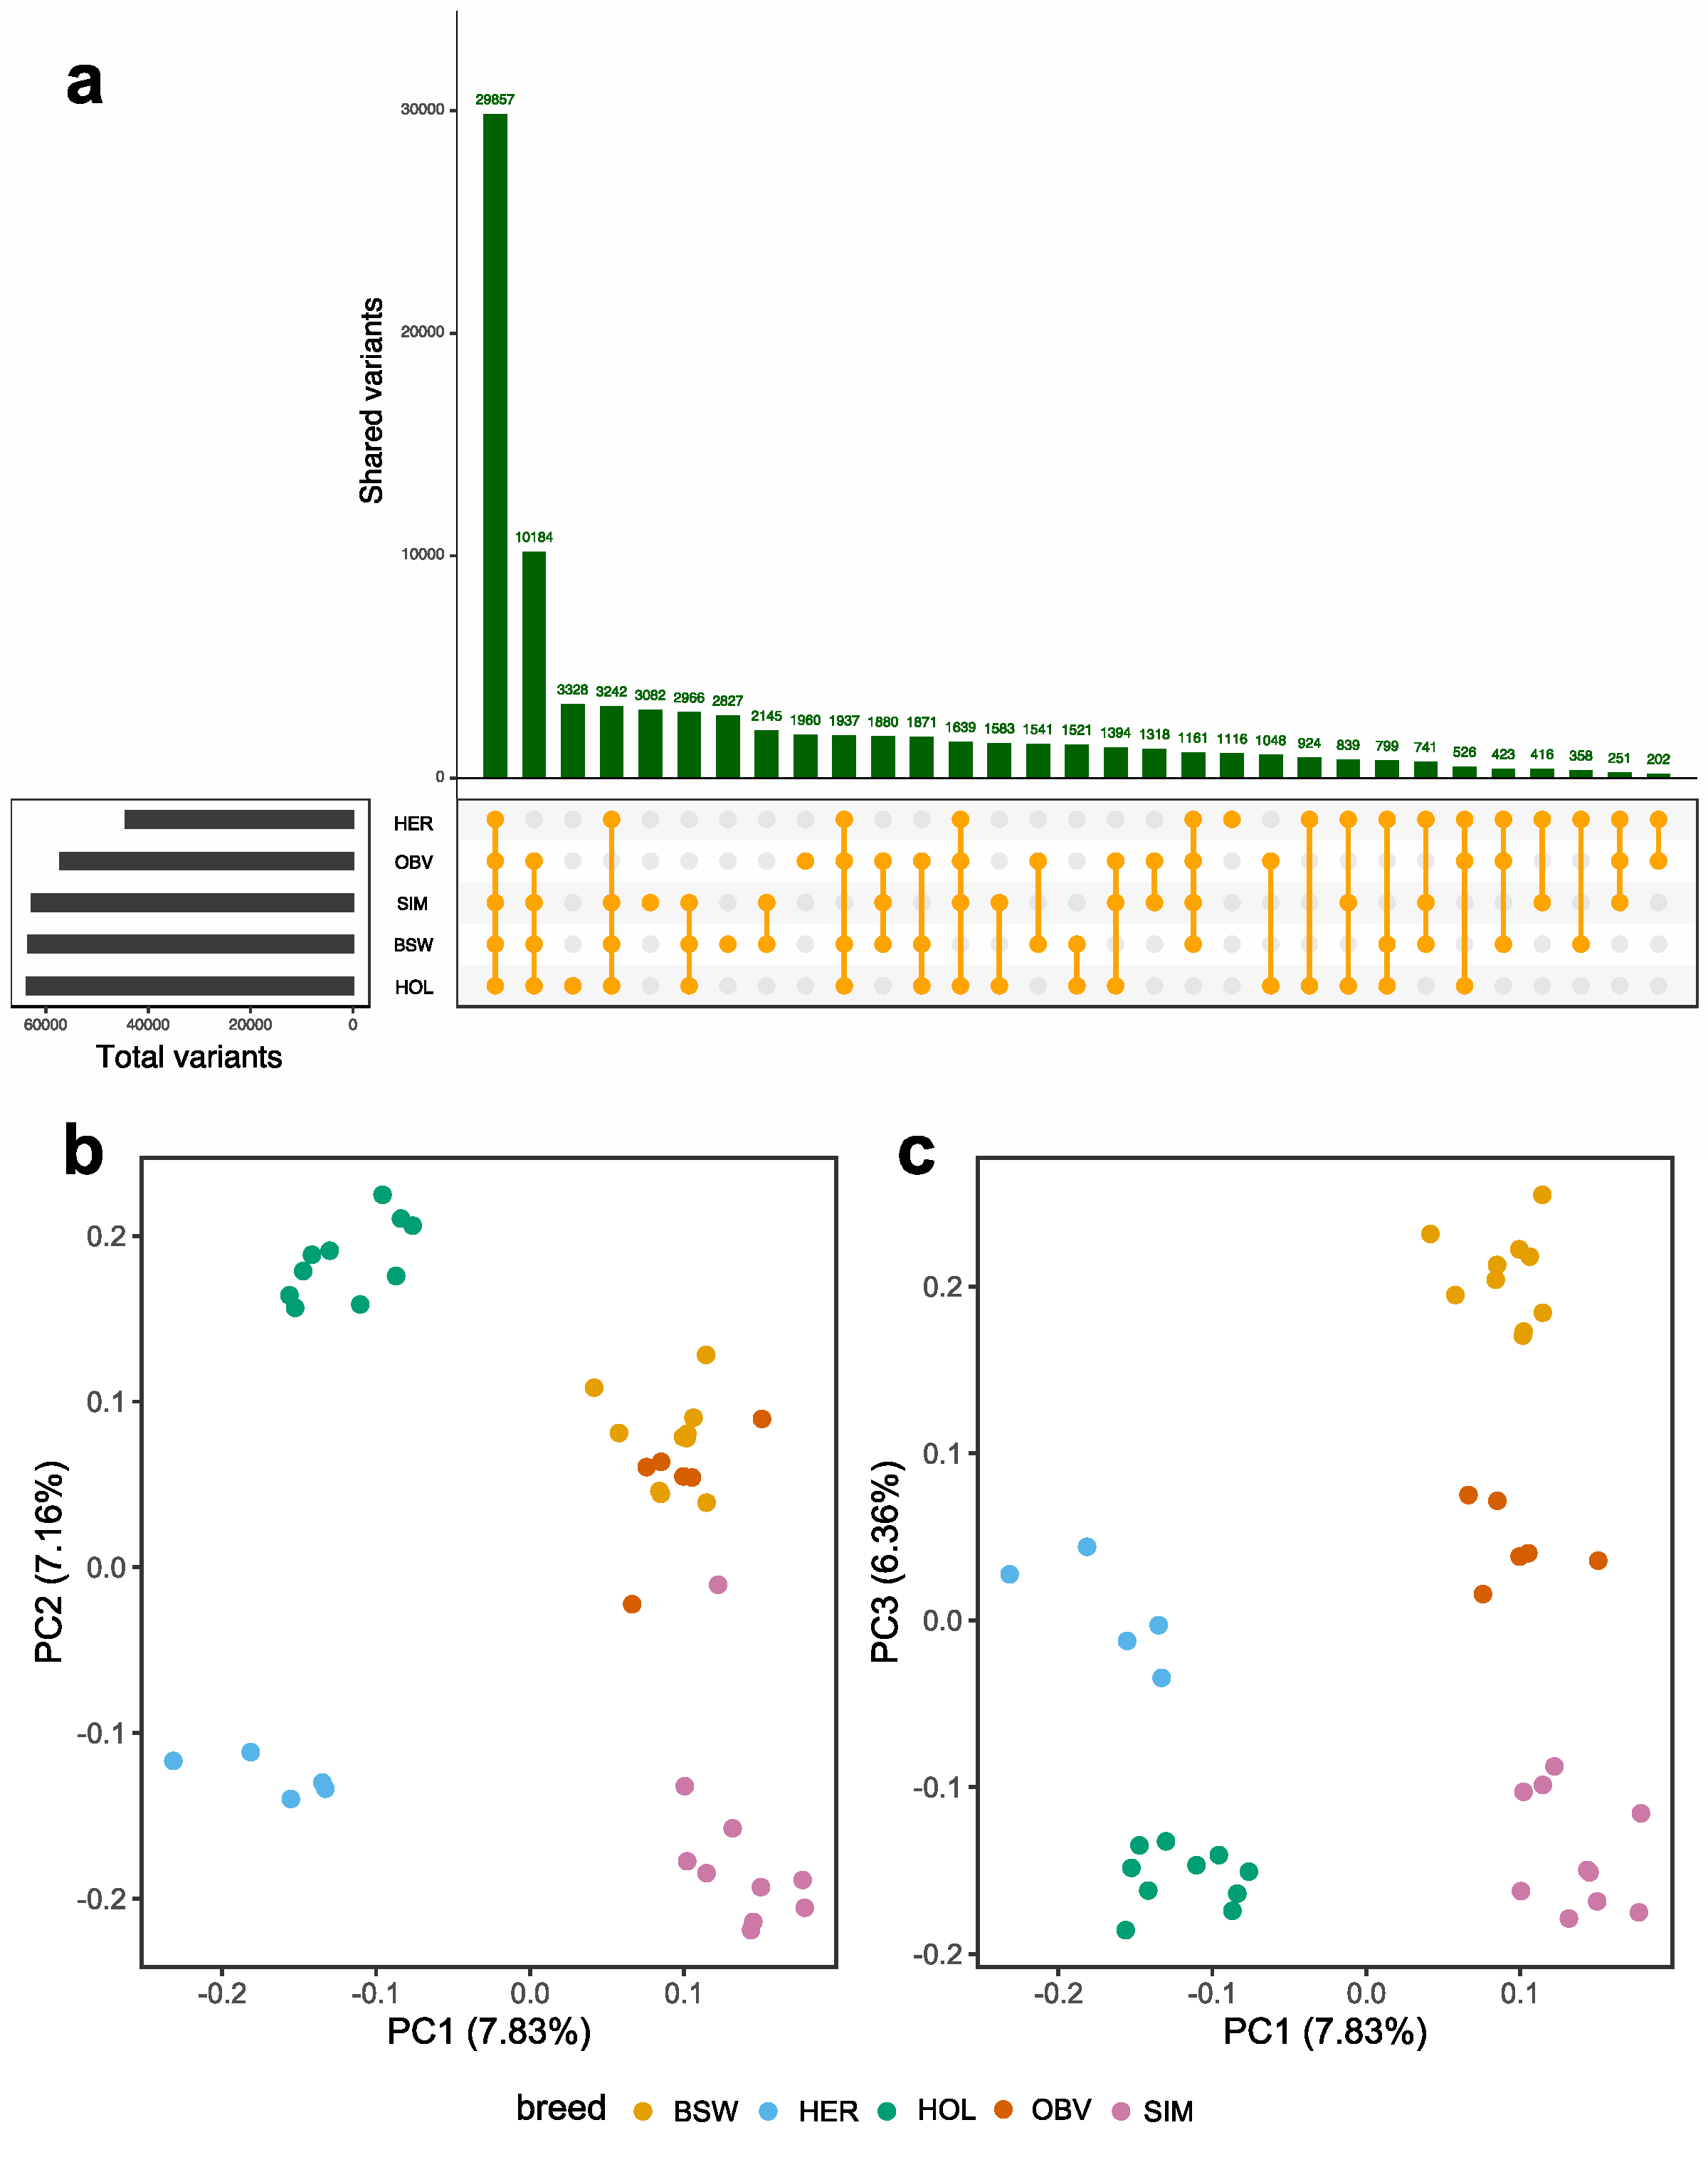
\includegraphics[width=\textwidth]{paper3/main_figure/Fig5.pdf}
        \caption[Variants detected from non-reference sequences]{\textbf{Polymorphic sites detected from non-reference sequences in five breeds.} \\
        \footnotesize{\textbf{(a)} Sharing of 83,250 variants across five taurine cattle breeds (BSW: Brown Swiss, HER: Hereford, HOL: Holstein, OBV: Original Braunvieh, SIM: Simmental). \textbf{(b, c)} The top three principal components (PC) of a genomic relationship matrix constructed from non-reference sequence variants separate the animals by breeds.}}
        \label{fig45:varnrf}
\end{figure}


\section{Discussion}

We utilize a bovine multi-assembly graph to uncover sequences that are not included in the Bos taurus reference genome. Novel contigs can also be assembled from unmapped reads, but placing them onto reference coordinates is difficult \citep{sherman2019assembly,golicz2016pangenome}. Our approach provides physical coordinates for the novel sequences because the breakpoints anchor them onto the reference genome. Despite including the genetically distant yak, constructing the multi-assembly graph using minigraph \citep{li2020design} was computationally efficient and scalable. Our multi-assembly graph utilizes a well-annotated backbone assembly to identify non-reference sequences from other assemblies. We show that the choice of the backbone as well as its genetic distance to all other assemblies influences the amount of non-reference bases uncovered through the multi-assembly graph. Sophisticated algorithms facilitate the reference-free alignment of thousands of assemblies \citep{armstrong2020progressive}. To determine the origin of the non-reference sequences, we developed an approach to assign labels to all nodes in the multi-assembly graph. Our evaluation showed that this strategy is highly accurate.

By systematically characterizing structural variations in multiple assemblies from domestic cattle and their close relatives, we detect 45,357 autosomal segments with a cumulative length of 70,329,827 bases that are novel when compared to the \emph{Bos taurus} reference genome. To obtain continuous non-reference sequences spanning multiple non-reference nodes, we recovered the non-reference alleles from structural variations. The number of bases detected in our study that are not in the \emph{Bos taurus }reference genome is comparable to values reported for pigs (72.5 Mb) \citep{tian2019building} and goats (38.3 Mb) \citep{li2019towards}, based on multi-assembly graphs constructed from 11 and 8 animals representing different breeds respectively. In our study, many non-reference sequences originate from yak. Hybridizing between yak and cattle is widely practiced, and results in fertile female descendants. However, multiple generations of backcrossing are required for males to resume fertility \citep{qi2010assessment}. A pangenome constructed from domestic cattle and their extant relatives as recently proposed by the Bovine Pangenome Consortium \citep{smith2020genome} will reveal variants that were lost during domestication and the separation of cattle into specialized breeds \citep{khan2020super}. For instance, some of the 8 million non-reference bases specific to Brahman might contribute to the adaptation of indicine cattle to harsh environments. Individual taurine assemblies also contain between 14 and 18 million bases that are missing in the Hereford-based reference assembly, many of which are shared between individuals. This value is somewhat higher than the 5-10 million non-reference bases detected per human genome \citep{ameur2018novo,audano2019characterizing,duan2019hupan}, possibly because cattle breeds diverged more strongly than human populations due to intense artificial selection. Each of the three taurine assemblies contains approximately 3 million autosomal non-reference bases that were not detected in any other assembly. There were also 4.4 million non-reference bases, of which 2.1 million were non-repetitive, that were present in all assemblies except the reference. This includes 1.2 million bases that are either specifically deleted in the Hereford breed or the animal used to build the reference, inadvertently propagating reference-bias.

A reference graph may integrate linear reference coordinates, non-reference sequences, and shorter variants \citep{hickey2020genotyping}. However, as many genome analysis tools still rely on a linear coordinate system, we append the novel non-reference sequences linearly to the ARS-UCD1.2 reference genome. Adding 100 bp flanking sequence on either side of the breakpoints facilitated accurate alignment of sequencing reads at the boundaries of the novel contigs. A graph-based approach might enable the mapping of sequencing reads spanning breakpoints \citep{hickey2020genotyping}. We considered only variations larger than 100 bp because integrating smaller variations increases the complexity of the resulting reference with limited benefit for downstream analyses \citep{li2020design}. We show that our extended ARS-UCD1.2 reference genome leads to improved DNA and RNA sequence read mapping in indicine and taurine cattle, even for breeds that did not contribute to the multi-assembly graph. However, excessively adding novel sequences to the reference genome carries the risk of increasing the number of ambiguous alignments.

The non-reference sequences comprise more repetitive elements than the overall ARS-UCD1.2 reference genome (76\% versus 48\%), but less than non-reference insertions detected from human pangenomes (88\%) \citep{sherman2019assembly,ameur2018novo}. Many non-reference sequences with repetitive elements were observed at immune gene complex loci, corroborating that these regions are highly repetitive \citep{schwartz2017evolution}. The immune gene complex loci also contain many non-repetitive non-reference sequences suggesting great allelic diversity which may cause assembly problems \citep{bakshy2021development}, thus resulting in gaps and missing sequences in the primary ARS-UCD1.2 assembly. 


We show that the 16.6 million non-repetitive non-reference bases encompass transcribed features. An \emph{ab initio} approach predicted 857 gene models from these sequences. The \emph{de novo} assembly of RNA sequencing read alignments from liver samples provided additional support for more than 400 of these gene models. As these analyses were only conducted on liver transcriptomes, it is highly likely that the non-reference sequences contain additional coding sequences that are transcribed in different tissues. The discovery of distinct putatively novel genes in an independent RNA sequencing dataset from peripheral blood leukocytes of Holstein cattle supports this hypothesis. Some of the putatively novel genes, including genes encoding olfactory receptors, were also present in the animal used to build the reference genome. Olfactory receptors have been observed to undergo frequent duplication and rapid evolution in mammalian genomes \citep{li2017comprehensive,hughes2018birth}. Segments encompassing duplicated genes may either be collapsed in primary assemblies or result in unplaced contigs that represent variants of the sequence in the assembled chromosomes \citep{vollger2019long,kelley2010detection}, hence the presence of paralogous copies among non-reference genes is expected. In order to obtain a confident set of non-reference genes, we retained only genes that were not expressed in Dominette. Many of the proteins encoded by these non-reference genes are predicted to play roles in the immune response. Pangenome analyses in species other than cattle have also revealed non-reference genes with immune-related functions \citep{li2017comprehensive,gordon2017extensive,golicz2020pangenomics}. Our findings show that more novel transcripts can be assembled in breeds that contribute to the multi-assembly graph (Brahman, Angus) than those not included (Holstein, Jersey), suggesting that individual assemblies contain breed-specific, functionally relevant bases. We detect the largest number of non-reference genes using RNA samples from Brahman, suggesting that breeds with great genetic distance from the reference benefit the most from a more diverse reference genome. Importantly, some putatively novel genes are differentially expressed between\emph{ Mycobacterium} bovis-infected and non-infected cattle, including genes that encode proteins that either contribute to the immune response against \emph{Mycobacterium} infections or may serve as targets for immunomodulation by the pathogen. These differentially expressed genes remained undetected when the transcriptomes were aligned against the standard linear reference genome \citep{mcloughlin2014rna}. Thus, our multi-assembly graph uncovers functionally active and biologically relevant genomic features that are missing in the Bos taurus reference genome.

Our extended reference genome also leads to substantial improvements over ARS-UCD1.2 in reference-guided alignment and variant discovery. First, the sequence read mapping rate increases for samples from all breeds investigated. Using the extended reference genome would enable mapping approximately 100K previously unmapped reads for samples sequenced at 30-fold coverage. Second, the mapping quality increases for reads that were previously aligned to other positions in ARS-UCD1.2, suggesting that the novel sequences resolve misalignments. These findings agree well with results from species other than cattle, including goats, pigs, and humans \citep{tian2019building,li2019towards,audano2019characterizing}. In addition, we show that the novel sequences contain polymorphic sites that remained hitherto undetected; we discover 83,250 variants that segregate within and between breeds of cattle. A cluster analysis based on these variants separated individuals by breed, suggesting that variable non-reference bases might be associated with breed-specific traits. This hypothesis is further supported by the “HIGH IMPACT” classification of 54 variants affecting non-reference bases. Considering that the Ti/Tv ratio of the variants in putatively novel coding sequences was only 1.83, they need to be scrutinized for false positives \citep{depristo2011framework}. In any case, our multi-assembly graph makes a previously neglected source of inherited variation amenable to genetic investigations.

The size of the bovine multi-assembly graph will grow as additional reference-quality assemblies from the Bovinae subfamily become available. Assemblies which are more distant will contribute correspondingly to the overall pangenome growth, increasing the flexible part of graph, and reducing the size of the core genome (\emph{SI Appendix}, \ref{sup_not:s42}). In its current implementation, our multi-assembly graph only contains insertions and deletions, as other types of structural variations (e.g., translocations, inversions) that distort the collinearity of the assembly graph cannot be integrated accurately with minigraph. We provide a versatile workflow that facilitates constructing and characterizing multi-assembly graphs for a flexible number of assemblies (\url{https://github.com/AnimalGenomicsETH/bovine-graphs}, \emph{SI Appendix}, \ref{sup_not:s45}). Our workflow provides tools to determine the origin of non-reference bases, derive structural variations from multi-assembly graphs, predict putatively novel genes and append the novel sequences linearly to a reference genome. We anticipate that the latter will become obsolete as soon as accurate and fast base-level alignment and split-read graph mapping enables the full-suite of genome analyses from a reference graph \citep{siren2020genotyping}.

\section{Methods}
\vspace{-1em}
\subsection*{Construction of the multi-assembly graph}

We used minigraph \citep{li2020design} (version 0.12-r389) with option \emph{-xggs} to integrate six reference-quality genome assemblies into a multi-assembly graph. The current bovine reference genome (Bos taurus taurus, ARS$-$UCD1.2, GCF\_002263795.1) and four assemblies that were generated previously are accessible at NCBI: Angus (\emph{Bos taurus taurus}, UOA\_Angus\_1, GCA\_003369685.2)\citep{low2020haplotype}, Brahman (\emph{Bos taurus indicus}, UOA\_Brahman\_1, GCF \_003369695.1) \citep{low2020haplotype}, Highland \emph{(Bos taurus taurus}, ARS\_UNL\_ Btau-highland\_paterna \_1.0\_alt, \\ GCA\_009493655.1) \citep{rice2020continuous}, yak (\emph{Bos grunniens}, \\ ARS\_UNL\_BGru\_maternal\_1.0\_p, GCA\_009493645.1) \citep{rice2020continuous}. Additionally, we constructed an assembly from a female Original Braunvieh calf (\emph{Bos taurus taurus}) using PacBio high-fidelity (HiFi) reads (\emph{SI Appendix}, \ref{sup_not:s41}). The sampling of blood from the Original Braunvieh animal and its parents was approved by the veterinary office of the Canton of Zurich (animal experimentation permit ZH 200/19).

The genetic distance among the six assemblies was estimated using Mash (version 2.2) \citep{ondov2016mash}. We performed genomic sketching separately for each assembly with \emph{mash sketch } using a sketch and $k$-mer size of s$=$1000 and $k$$=$21, respectively. Sketches were combined using \emph{ mash paste}, and \emph{mash dist} was used to estimate the distances between the assemblies. A phylogenetic tree was built from the estimated pairwise distances using the neighbor-joining method \citep{saitou1987neighbor} as implemented in the R package ape (version 5.4) \citep{paradis2019ape}. The tree was visualized with the \emph{phylo.plot} function, using the yak assembly as the outgroup to root the tree.

\subsection*{Identification of non-reference segments from the multi-assembly graph}

We refer to nodes that are not in the Hereford-based reference genome (ARS-UCD1.2) as non-reference nodes. We separately aligned (with minigraph parameters “--cov -x asm”) each of the six assemblies back to the multi-assembly graph to determine the support for non-reference nodes. For each alignment, all nodes with non-zero coverage, i.e., nodes traversed by this specific assembly, were labelled. After iterating through all the alignments, each node then contained labels for every assembly which passed through it. As such, each node necessarily had at least one label, while a node traversed by all six assemblies would have six labels (\emph{SI Appendix}, Fig. \ref{sup_fig:s41}).

It was possible to assess minigraph’s alignment accuracy for the path of the Hereford-based reference genome (ARS-UCD1.2), because all reference nodes in the multi-assembly graph were from this assembly. Nodes were considered true positive (TP) and true negative (TN) when reference and non-reference nodes were correctly assigned Hereford labels, respectively. Reference nodes aligned as non-reference nodes were assigned false negative (FN) and non-reference nodes aligned as reference nodes were assigned false positive (FP). We characterized alignment recall (TP / (TP+FN)), precision (TP / (TP+FP)), and overall F1 score (2 * (precision * recall) / (precision + recall)).

\subsection*{Identification of structural variations from the multi-assembly graph}

We used the bubble popping algorithm of gfatools (version 0.4) \citep{li2020design} to derive the structural variations from the multi-assembly graph. In the reference graph model of minigraph, a bubble is a branching region in the graph for which the start and end node are reference sequences. A path traversing the start and end nodes represents an allele of a structural variant. 

The version of gfatools considered in our study reports the shortest and longest path for each bubble. To detect and classify all paths within a bubble, we applied the following stepwise procedure (\emph{SI Appendix}, Fig. \ref{sup_fig:s42}):

\begin{itemize}
    \item Determine the start and stop node for each bubble using the bubble popping algorithm of gfatools.
    \item Traverse all possible paths in the bubble using a recursive depth-first search.
    \item Retain only paths with color-consistent labels (see above).
    \item Classify a path as a reference path when all nodes and edges are part of the Hereford-based reference assembly, and as non-reference otherwise.
    \item Compare reference and non-reference paths to classify the type of the structural variations.
\end{itemize}


Structural variations were classified as biallelic if two paths were observed in a bubble and multi-allelic if a bubble contained more than two paths. The structural variations were further classified into:

\begin{itemize}
    \item Alternate deletion, when the non-reference path was shorter than the reference path (but the reference path has nonzero length).
    \item Complete deletion, when the non-reference path has a length of zero.
    \item Alternate insertion, when the non-reference path was longer than the reference path.
    \item Complete insertion, when the reference path has a length of zero.
\end{itemize}

Breakpoints of structural variations were determined according to ARS-UCD1.2 reference coordinates. We overlapped the breakpoints with annotations from Ensembl (build 101) to identify structural variations in coding sequences. Affected genes were subjected to a gene set enrichment analysis using PANTHER (\url{http://pantherdb.org/}) \citep{mi2019panther} for which the Bos taurus reference gene list was supplied as a baseline. 

To validate the structural variations, we mapped 6,803,270 ($~$46-fold coverage) PacBio HiFi reads to the multi-assembly graph using GraphAligner (version 1.0.12) \citep{rautiainen2020graphaligner} with preset -x vg (variation graph mapping). The HiFi reads were generated from a Nellore x Brown Swiss crossbred bull (SAMEA7765441), representing taurine and indicine breeds that were not used to build the multi-assembly graph. The veterinary office of the Canton of Zurich approved the sampling of blood from the crossbred animal and its parents (animal experimentation permit ZH 200/19). The mean read length was 20,612 bases with an average accuracy of 99.76\%. We calculated coverage (number of reads aligned) at each node and edge in the graph based on the GAF (Graphical Alignment Format) output from GraphAligner.  

We combined all non-reference alleles (excluding complete deletions, paths without non-reference bases, and paths with length less than 100 bp) to obtain a comprehensive set of non-reference bases from the multi-assembly graph. To facilitate the mapping of short reads to the segment edges, we added 100 bp of flanking sequences (derived from sequences at the source and sink nodes) on either side of the structural variations. The flanking sequences were not considered for length calculations or gene predictions (see below). 

To investigate the repeat content of the non-reference sequences, we used the RMBlastn search engine (version 2.10.0) to run RepeatMasker version 4.1.1 (option -species cow) \citep{Smit2015} using the database of repetitive DNA elements from Repbase (release 20181026) \citep{bao2015repbase}.  

\subsection*{Bioinformatic characterization of non-reference sequences}

In order to reveal functionally active non-reference sequences, we performed two complementary analyses: 

First, we compared the repeat masked non-reference sequences against a local protein database using DIAMOND BLASTX (version 0.9.30) \citep{buchfink2015fast}. Using DIAMOND makedb, the local protein database was built from the RefSeq protein sequences of

\begin{itemize}
\item Taurine cattle (\emph{Bos taurus taurus}, GCF\_002263795.1\_ARS-UCD1.2\_protein.faa)
\item Indicine cattle (\emph{Bos taurus indicus}, GCF\_003369695.1\_UOA\_Brahman\_1\_protein.faa)
\item Yak (\emph{Bos mutus}, GCF\_000298355.1\_BosGru\_v2.0\_protein.faa)
\item Human (\emph{Homo sapiens}, GCF\_000001405.39\_GRCh38.p13\_protein.faa)
\item Mouse (\emph{Mus musculus}, GCF\_000001635.26\_GRCm38.p6\_protein.faa)
\item Bison (\emph{Bison bison,} GCF\_000754665.1\_Bison\_UMD1.0\_protein.faa)
\item Water buffalo (\emph{Bubalus bubalis}, GCF\_003121395.1\_ASM312139v1\_protein.faa)
\item Goat (\emph{Capra hircus}, GCF\_001704415.1\_ARS1\_protein.faa)
\item Sheep (\emph{Ovis aries}, GCF\_002742125.1\_Oar\_rambouillet\_v1.0\_protein.faa)
\item the curated protein databases of SwissProt and PDB (\url{ftp://ftp.ncbi.nlm.nih.gov/blast/db/FASTA/}) 
\end{itemize}


To query the non-reference sequences against the local protein database we ran BLASTX with the parameters “--more-sensitive --e-value 1e-10 --outfmt 6”. We considered only the top hit for each queried sequence with minimum coverage and identity of 80\%.

Second, we performed an ab initio gene structure prediction from the repeat masked non-reference sequences using a local instance of Augustus (version 3.3.3) \citep{stanke2003gene} using default parameters trained on the human genome. From the Augustus GTF output file, we extracted the number of gene models, the number of gene models with transcription start and termination site, transcript length, exon count, and length per gene, coding sequence count and length per gene, and protein length of the putatively novel protein-coding sequences. To classify the domain and family of the putatively novel proteins, we converted the Augustus GTF output to the fasta format and performed a query against the local protein database (as above) using DIAMOND BLASTP with the same parameters and thresholds as the BLASTX query.

\subsection*{\emph{De novo} transcript assembly from non-reference sequences}

We downloaded between 12,361,440 and 34,421,106 paired-end RNA-sequencing reads from liver tissue from 10 Angus \citep{xiang2018genome}, 10 Brahman \citep{nguyen2016p1012}, 9 Holstein and 10 Jersey \citep{salleh2018gene} cattle, as well as from Dominette - the animal used to construct the ARS-UCD1.2 reference genome \citep{rosen2020novo}. Adapter sequences and low-quality bases were removed from the raw RNA sequencing data using default parameters of fastp (version 0.19.4) (60). The filtered reads were then aligned using HISAT2 (version 2.1.0) \citep{kim2019graph}, with option “--dta” to facilitate the downstream transcriptome assembly, to the original ARS-UCD1.2 reference as well as the extended version of the ARS-UCD1.2 reference. The extended reference was constructed by appending repeat masked non-reference sequences as unplaced contigs.  

Putative novel transcripts were assembled \emph{de novo} using StringTie2 (version 2.1.1) \citep{kovaka2019transcriptome} from RNA-seq reads that aligned to the non-reference sequences. To facilitate transcript assembly, we supplied the ARS-UCD1.2 Ensembl annotation (build 101) and the novel gene models predicted by Augustus (see above). Transcripts were assembled \emph{de novo} separately for all RNA sequencing samples. Subsequently, we used StringTie2 \emph{merge} to create a unique set of transcripts across all samples and facilitate the assembly of full-length transcripts from partially assembled transcripts. We quantified gene expression for each sample with StringTie2 using a fixed (merged) GTF file that was generated previously (without predicting novel transcripts, option -e). Gene abundance was quantified in transcript per million (TPM).  

\subsection*{Differential gene expression analysis}

We utilized publicly available peripheral blood leukocyte transcriptomes of eight \emph{Mycobacterium bovis}-infected and eight age-matched healthy Holstein cattle \citep{mcloughlin2014rna} to detect differentially expressed genes from non-reference sequences. The RNA-sequencing data contain between 9,272,629 and 25,358,979 single-end reads of length 78 bp. We performed quality control on the raw sequencing reads using fastp (version 0.19.4) \citep{chen2018fastp} with default parameters. The filtered reads were then mapped to the extended ARS-UCD1.2 reference genome that contained the non-reference sequences using HISAT2 \citep{kim2019graph}. Potential non-reference transcripts were assembled \emph{de novo} with StringTie2 (see above). Gene-level read counts were estimated based on a custom annotation file that contained the Ensembl (build 101) ARS-UCD1.2 genome annotation and the non-reference annotation as generated by StringTie2 using the \emph{featurecounts} function of the Rsubread package (option countMultiMappingReads =FALSE to exclude multi-mapping reads). The read count matrix was used as input for EdgeR version 3.24.3 \citep{robinson2010edger}. We normalized transcript abundance by sequencing depth using the trimmed-mean of M-values (TMM) approach. Genes that were expressed at ≥1 count per million (CPM) in at least eight samples were tested for differential expression in peripheral blood leukocytes between \emph{Mycobacterium bovis}-infected and control animals using a generalized linear model (GLMQfit) with dispersion parameter estimated using the Cox-Reid method. Genes were considered to be differentially expressed at a Benjamini-Hochberg-corrected FDR≤0.05. Multidimensional scaling of the normalized read count matrix of the differentially expressed genes was performed using the \emph{cmdscale} function in R.

\subsection*{Mapping and variant calling from whole-genome short read data}

We considered the original ARS-UCD1.2 reference genome and an extended version of the reference that additionally contained 70,329,827 non-reference bases detected from five assemblies. We used paired-end short read sequencing data from 45 samples representing five breeds: Original Braunvieh, Brown Swiss, Holstein, Simmental \citep{hafliger2020il17ra}, and Hereford (including Dominette, the animal used to construct the ARS-UCD1.2 reference genome) \citep{rosen2020novo,young2020genomic} that had average sequencing coverage of 18.94-fold. Quality control of the short-read sequencing reads was performed using fastp (version 0.19.4) \citep{chen2018fastp} with default parameter settings. The filtered reads were subsequently mapped to the original ARS-UCD1.2 reference and the extended ARS-UCD1.2 reference that also contained non-reference sequences using the mem-algorithm of BWA (version 0.7.17) \citep{li2013aligning} with default parameters. Duplicate reads were marked with Samblaster (version 0.1.24) \citep{faust2014samblaster}. 

We performed multi-sample variant calling (SNP and Indels) on the non-reference sequences using SAMtools (version 1.10) \citep{li2009sequence} and GATK (version v4.1.9.0) \citep{poplin201178others} as detailed in \citet{crysnanto2019accurate}. Base quality scores were recalibrated using known variants from the 1000 bull genomes project database (\url{http://www.1000bullgenomes.com/doco/ARS1.2PlusY_BQSR_v3.vcf.gz}). We applied the GATK modules \emph{HaplotypeCaller}, \emph{GenomicsDBImport} and \emph{GenotypeGVCFs} to discover and genotype polymorphic sites. The variants were subsequently hard-filtered using recommended parameters (SNP filters: $QD < 2 || QUAL < 30 || FS > 60 || MQ < 40 || MQRankSum < -12.5 || ReadPosRankSum < -8 || AN < 10$, Indel filters: $QD < 2 || QUAL < 30 || FS > 200 || ReadPosRankSum < -20.0 || AN < 10)$ \citep{crysnanto2019accurate}. A second independent variant discovery and genotyping approach was performed using SAMtools mpileup and bcftools call \citep{li2009sequence}. The resulting genotypes were subsequently hard-filtered according to parameters recommend by the 1000 bulls genomes project ($QUAL < 20 || MQ < 30 || DP < 10 || AN < 10$) \citep{daetwyler2014whole}. To create a consistent variant representation across both datasets, variants were normalized using vt (version 0.5) \citep{tan2015unified}. We retained only filtered variants, which were identified by both SAMtools and GATK. Functional consequences of variants affecting non-reference bases were predicted based on the GTF-file from Augustus (see above) using Ensembl’s Variant Effect Predictor \citep{mclaren2016ensembl}.

\subsection*{Data availability}

Short sequencing reads are available at the European Nucleotide Archive (ENA) (\url{http://www.ebi.ac.uk/ena}) with study accession PRJNA436715 (Transcriptome - Brahman), PRJNA392196 (Transcriptome - Angus), PRJNA357463 (Transcriptome – Holstein, Jersey), PRJNA294306 (Transcriptome - Dominette), PRJNA257841 (Differential expression analysis – Holstein), PRJEB18113 (WGS – BSW, OBV, HOL, SIM), PRJNA494431 (WGS - Hereford), PRJNA391427 (WGS - Dominette). PacBio HiFi reads for an Original Braunvieh animal used to construct a \emph{de novo} assembly are available at study accession PRJEB42335 under sample accession SAMEA7759028. PacBio HiFi reads for a Nelore x Brown Swiss bull are available at study accession PRJEB42335 under sample accession SAMEA7765441. Data supporting this study, including the multi-assembly graph, non-reference sequences, putatively novel genes, transcript abundances and sequence variants detected from non-reference sequences are available via Zenodo (\url{https://doi.org/10.5281/zenodo.4385983}) \citep{Crysnanto2021}. 

\subsection*{Code availability}

Workflows to construct multi-assembly graphs and custom scripts to characterize non-reference sequences are available via \emph{Github} (\url{https://github.com/AnimalGenomicsETH/bovine-graphs}). All workflows were built using Snakemake (version 5.30.1)and custom scripts were written in R (version 3.5.1) \citep{RCoreTeam2017} and Python (version 3.7.1). 

\subsection*{Acknowledgements}

We are thankful for the excellent technical support provided by the ETH Zürich functional genomics platform FGCZ (\url{https://fgcz.ch/}). Computing was done at the Leonhard High Performance Compute cluster at ETH Zürich. This study was supported by grants from the Swiss National Science Foundation (310030\_185229) and the Swiss Federal Office for Agriculture (FOAG), Bern.

\vspace{-2em}

\singlespacing
\footnotesize

\renewcommand{\bibname}{References \vspace{-1em}}
\bibliographystyle{unsrtnat}
\bibliography{references/chapter4_ref}

\ifdefined\BuildingFromMainFile
\else
   \end{document}
\fi